\documentclass[journal,transmag]{IEEEtran}
    \usepackage{algorithm}
    \usepackage{graphicx}
    \usepackage{verbatim}
    \usepackage{pythonhighlight}
    \usepackage{listings}

    \hyphenation{op-tical net-works semi-conduc-tor}
    \begin{document}
    \title{ Analysis and Comparison of Brute-Force and Genetic Algorithm methods
        on Traveling Salesman Problem }

    \author{ \IEEEauthorblockN{Onur Temizkan} \IEEEauthorblockA{ Department of
        Computer Engineering, Izmir Institute of Technology, Urla / Izmir /
        Turkey } }

    \markboth{Optimization Methods Term Project, Onur Temizkan, May 2018}{}%

    \IEEEtitleabstractindextext{%
    \begin{abstract}
        \textit{ Abstract: Traveling Salesman Problem (TSP) is a common
            NP-Complete problem in Computer Science and Optimization. Thus,
            there is no known way to solve it in polynomial time at the time of
            this writing. In this report, I will analyse Genetic algorithm
            approach to TSP and compare it with Brute-Force Search method. }
    \end{abstract}

    \begin{IEEEkeywords}
    traveling salesman problem, optimization, genetic algorithm, TSP,
    combinatorics.
    \end{IEEEkeywords}}

    \maketitle
    \IEEEdisplaynontitleabstractindextext \IEEEpeerreviewmaketitle

    \section{Introduction}

    \IEEEPARstart{I}{n} this report, The performance of a genetic algorithm
    implementation will be analyzed, onto Traveling Salesman Problem to find
    the optimum path to traverse a multi-node undirected and weighted graph. On
    the other side, to measure the pros / cons of the GA, brute-force method
    will also be applied on the same problem. The problem definitions and
    solutions are implemented in Python.

    \section{Problem Definition}

    For this research, the problem is defined as a \textit{undirected graph}
    with \textit{N} nodes. There are edges with several weights between those nodes. In
    TSP analogy, the nodes represent cities, and edges represent paths between
    those cities. Edge weights, represent the distances between two cities. A
    route is valid if the salesman start traveling from a given node, visit all
    cities once, and return back to the starting city.

    Since the graph is not necessarily a \textit{complete graph}, the algorithm
    should check next available nodes from the node at a single time to create
    the route. All nodes should be visited once. So the implementation should be
    aware of the possible circular routes and should avoid them.

    Moreover, since the graph edges are weighted by definition, the algorithms we
    implement should select from possible routes in awareness of costs.

    The TSP that will be solved is shown in Figure \ref{fig:tsp-problem}

    \begin{figure}[h!]
        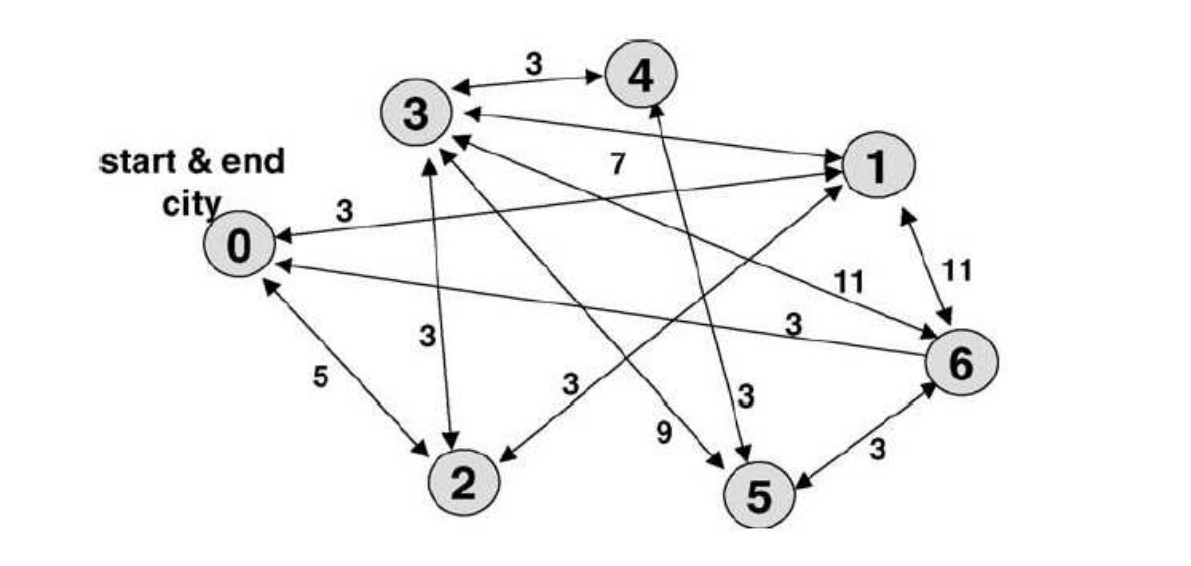
\includegraphics[width=\linewidth]{tsp.png}
        \caption{TSP to be solved}
        \label{fig:tsp-problem}
    \end{figure}


    \section{Methods}

    In this paper, two different methods will be applied to the same problem.

    \subsection{Brute-Force Search}

    Brute-Force Search solves this problem in an inefficient but a definite way.
    To find the best route, Brute-Force Search checks all possible path
    permutations without any specific condition or restriction. While checking
    routes, it stores and updates the shortest route from the start of the
    execution. When the checks are finished, the shortest route is the last
    route stored. Since it checks all possible routes, it makes sure that the
    returned result is the best possible solution. This implementation is very
    memory-efficient because only thing that is stored, is the shortest path and
    its size.

    \subsection{Genetic Algorithm}

    Solving the problem with a Genetic Algorithm is more efficient but
    indefinite. This is because in a GA, it's not necessary to check all
    possible routes. Instead, evolving a set of routes is tried to create a
    better route. GA approach is an iterative method which is based on the
    natural selection mechanism of evolution. Since natural selection
    \textit{-thus evolution} doesn't have a stopping point, Genetic Algorithms
    do not have a strict finishing point. So it's presumed that there can always be
    a better solution at the any state of the algorithm execution, and a
    stopping condition should be chosen.

    \begin{algorithm} % enter the algorithm environment
        \textit{1.} Create a population with \textit{N} random routes. \\
        \textit{2.} Select the best \textit{k} routes \\
        \textit{3.} combine / match the selected routes to create an ancestor
        route. \\
        \textit{4.} Mutate that ancestor node \textit{N-1} times to create a new
        generation with N new routes. \\
        \textbf{Repeat} steps \textit{2} to \textit{4}, \\
        \textbf{Until} the best route hasn't been changing for x generations \\
        \textit{5.} Return the best route and its length.


        \caption{Genetic Algorithm on TSP} % give the algorithm a caption
        \label{alg2} % and a label for \ref{} commands later in the document

    \end{algorithm}

    \section{Implementation}

    The code \cite{code_repository} of both Brute-Force and Genetic Algorithm
    approaches are implemented in Python. We tried to keep the code simple by
    removing any nonessential parts. This also helped to measure and compare the
    performances since there are almost no avertible computational cost in any
    of those two implementations.

    Python definition and representation of the TSP is shown below in Figure
    \ref{fig:data-definition}:

    \begin{figure}[h!]
        \begin{python}
PATH_DEF = {
    0: [(1, 3), (2, 5), (6, 3)],
    1: [(0, 3), (2, 3), (3, 7), (6, 11)],
    2: [(0, 5), (1, 3), (3, 5)],
    3: [(1, 7), (2, 3), (4, 3), (5, 9), (6, 11)],
    4: [(3, 3), (5, 3)],
    5: [(3, 9), (4, 3), (6, 3)],
    6: [(0, 3), (1, 11), (3, 11), (5, 3)]
}
        \end{python}
        \caption{TSP Data Definition}
        \label{fig:data-definition}
    \end{figure}

    An excerpt from Brute-Force implementation is given below.
    \begin{figure}[h!]
        \begin{python}
def trav_salesman():
    for point in PATH_DEF:
        find_all_paths([point])

    min_length = inf
    min_path = None

    for path in all_paths:
        path_length = calc_path_length(path)
        if path_length < min_length:
            min_path = path
            min_length = path_length
        \end{python}
        \caption{Brute Force Implementation}
    \end{figure}

    Since our test example is an incomplete undirected graph, our genetic implementation
    is based on specifically for that kind of graphs, another implementation for
    complete graphs can be also found in given repository. \cite{code_repository}

    \begin{figure}[h!]
        \begin{python}
def trav_salesman():
    population = pre_populate()

    for i in range(MAX_GENERATIONS):
        fittest = get_fittest(population)
        (fittest_path, fittest_length) = fittest

        all_generation_fittest_lengths.append(
            fittest_length
        )
        all_generation_average_lengths.append(
            get_average(population)
        )
        all_generation_worst_lengths.append(
            get_worst(population)[1]
        )

        population = populate(fittest_path)
        \end{python}
        \caption{Genetic Algorithm Implementation}
    \end{figure}


    \section{Results}
    \subsubsection{First Trial}
    In the first implementations of these two algorithms, the results were
    interesting. Genetic Algorithm took more time than Brute-Force
    implementation which was unexpected. The results are shown in
    Table 1.

    \begin{table}[h!]
        \begin{center}
            \begin{tabular}{| l | l | l |}
            \hline
            & Brute Force & Genetic Algorithm \\ \hline
            Iters / Gens & 102 & 7 \\ \hline
            Path & [0, 6, 5, 4, 3, 2, 1] & [3, 2, 1, 0, 6, 5, 4] \\ \hline
            Distance & 18 & 18 \\ \hline
            Time (sec.) & 0.00134 & 0.0024 \\
            \hline
            \end{tabular}
        \end{center}
        \caption{Compared Execution Results of First Implementation}
    \end{table}

    The reason of this would be the mutation logic and sample size selection.
    Since the used problem size was very small, that implementation had unneeded
    results.

    So, the implementation should have been changed. \\

    \subsubsection{Second Trial}
    A new implementation with update sample size and changed mutation logic
    (which includes combining best routes at any time), gave better results. The
    new result are shown in Figure 5 and Table II.

    \begin{figure}[h!]
        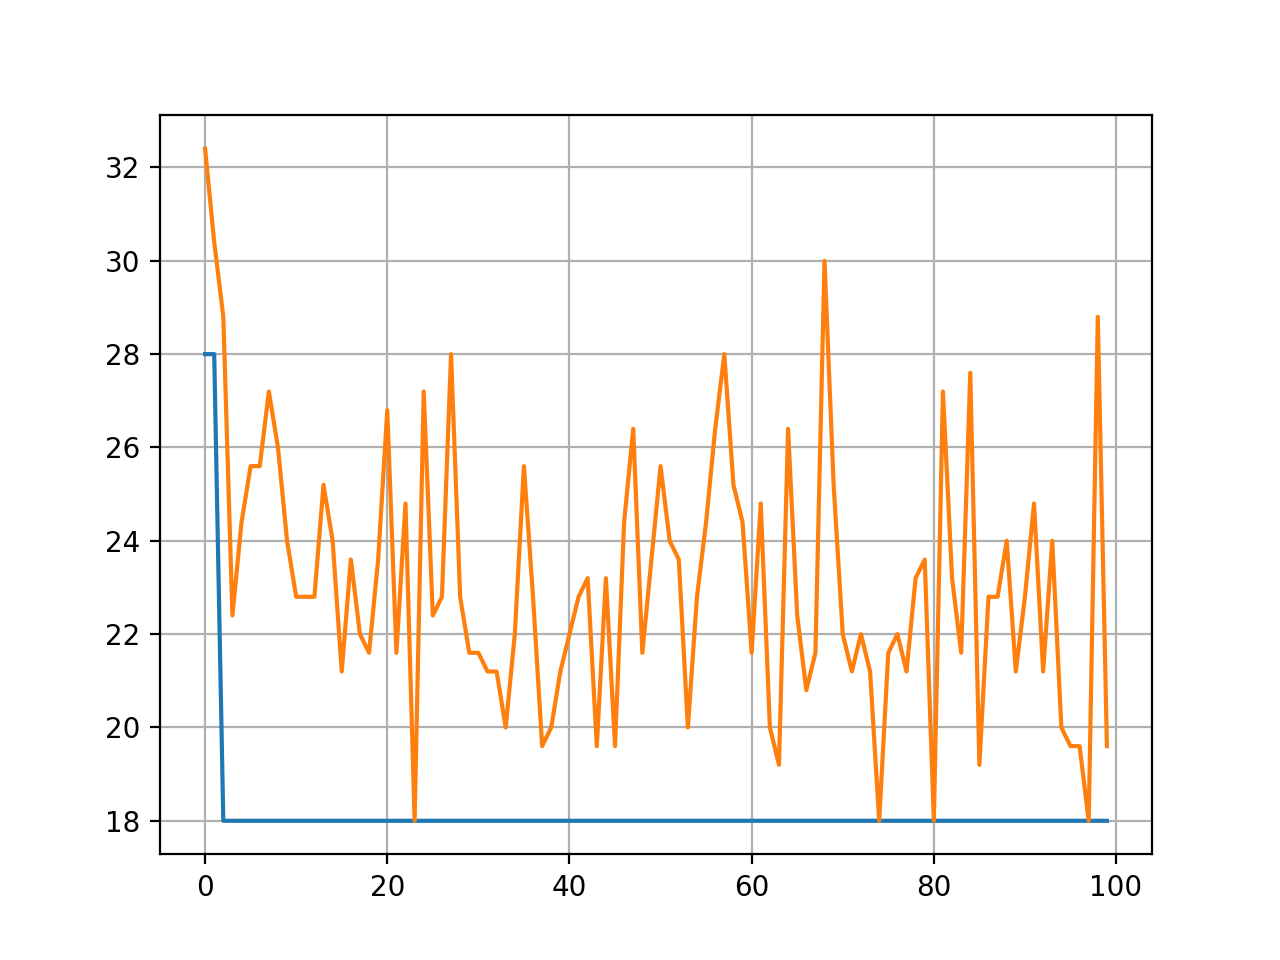
\includegraphics[width=\linewidth]{new-results.png}
        \caption{
            New results showing best route sizes in a generation in blue, and
            mean size of a generation in orange.
        }
        \label{fig:new-results}
    \end{figure}

    \begin{table}[h!]
        \begin{center}
            \begin{tabular}{| l | l | l |}
            \hline
            & Brute Force & Genetic Algorithm \\ \hline
            Iters / Gens & 102 & 2 \\ \hline
            Path & [0, 6, 5, 4, 3, 2, 1] & [3, 2, 1, 0, 6, 5, 4] \\ \hline
            Distance & 18 & 18 \\ \hline
            Time (sec.) & 0.00134 & 0.00037 \\
            \hline
            \end{tabular}
        \end{center}
        \caption{Compared Execution Results of Second Implementation}
    \end{table}

    As can be seen, the new implementation of Genetic Algorithm Solution, the
    execution time got smaller and the result is found in the second generation.
    Also, interestingly the found solution of the GA implementation is exactly
    the same as the first implementation results.
    \section{Conclusion}

    Genetic Algorithm approach works very well on Traveling Salesman Problem.
    That approach significantly reduced the number of iterations to find the
    optimal route, comparing with the Brute-Force Search. Although, our sample
    problem is not so big, it reduced the execution time in a significant
    amount. When the problem gets bigger, the execution time benefits should be
    much more significant. And note that this implementation is only a solution
    for incomplete graph based TSPs. For other TSP domains like coordinate
    systems, other implementations and logic should be found. A sample
    implementation of these kind of problems can also be found in
    \cite{code_repository}.

    \ifCLASSOPTIONcaptionsoff
      \newpage
    \fi

    \begin{thebibliography}{1}

    \bibitem{code_repository}
    http://github.com/onurtemizkan/tsm-genetic-algorithm
    \end{thebibliography}

    \end{document}
